\subsubsection{22.11.14 (Соревнования)}
\begin{center}
	2-ой день соревнований "Робофест-Юг"
\end{center}
Сегодня проходили квалификационные матчи и защита инженерных книг.
\newline 
Результаты матчей: 2 победы из 4. 
\newline
Результаты защиты инженерной книги пока неизвестны.
\newline
Основные проблемы, выявленные в ходе матчей:
\begin{enumerate}
	\item Из-за недостаточного уделения времени тренировкам, в ходе матчей мы неточно забрасывали мячи в подвижные корзины. 
	
	\item Поскольку провод сервопривода, отвечающего за опрокидывание ковша, был плохо закреплен на подъемнике, он часто зацеплялся за движущиеся части мебельных реек и рвался, из-за чего связь с сервоприводом терялась и закидывать мячи в корзины становилось невозможно.
	
\end{enumerate} 
Внесенные  доработки:
\begin{enumerate}
	\item Была написана программа для автономного периода, включавшая в себя съезд робота с пандуса и забрасывание автономных мячей в 60-ти сантиметровую корзину.
	
	\item Также была реализована программа автономного периода из зоны парковки. Она позволяла сбивать упор в случае, если он находился в одном положении из трех возможных.
	
	\item Из-за чрезмерных нагрузок, которые испытывали перекладины подъемника, одна из них погнулась и мы были вынуждены укрепить ее трубкой большего диаметра. Это улучшило ситуацию, однако было решено, что по возвращении с соревнований мы заменим те из перекладин, которые испытывают наибольшие нагрузки, с алюминиевых на стальные.
	
%	\begin{figure}[H]
%		\begin{minipage}[h]{0.2\linewidth}
%			\center  
%		\end{minipage}
%		\begin{minipage}[h]{0.6\linewidth}
%			\center{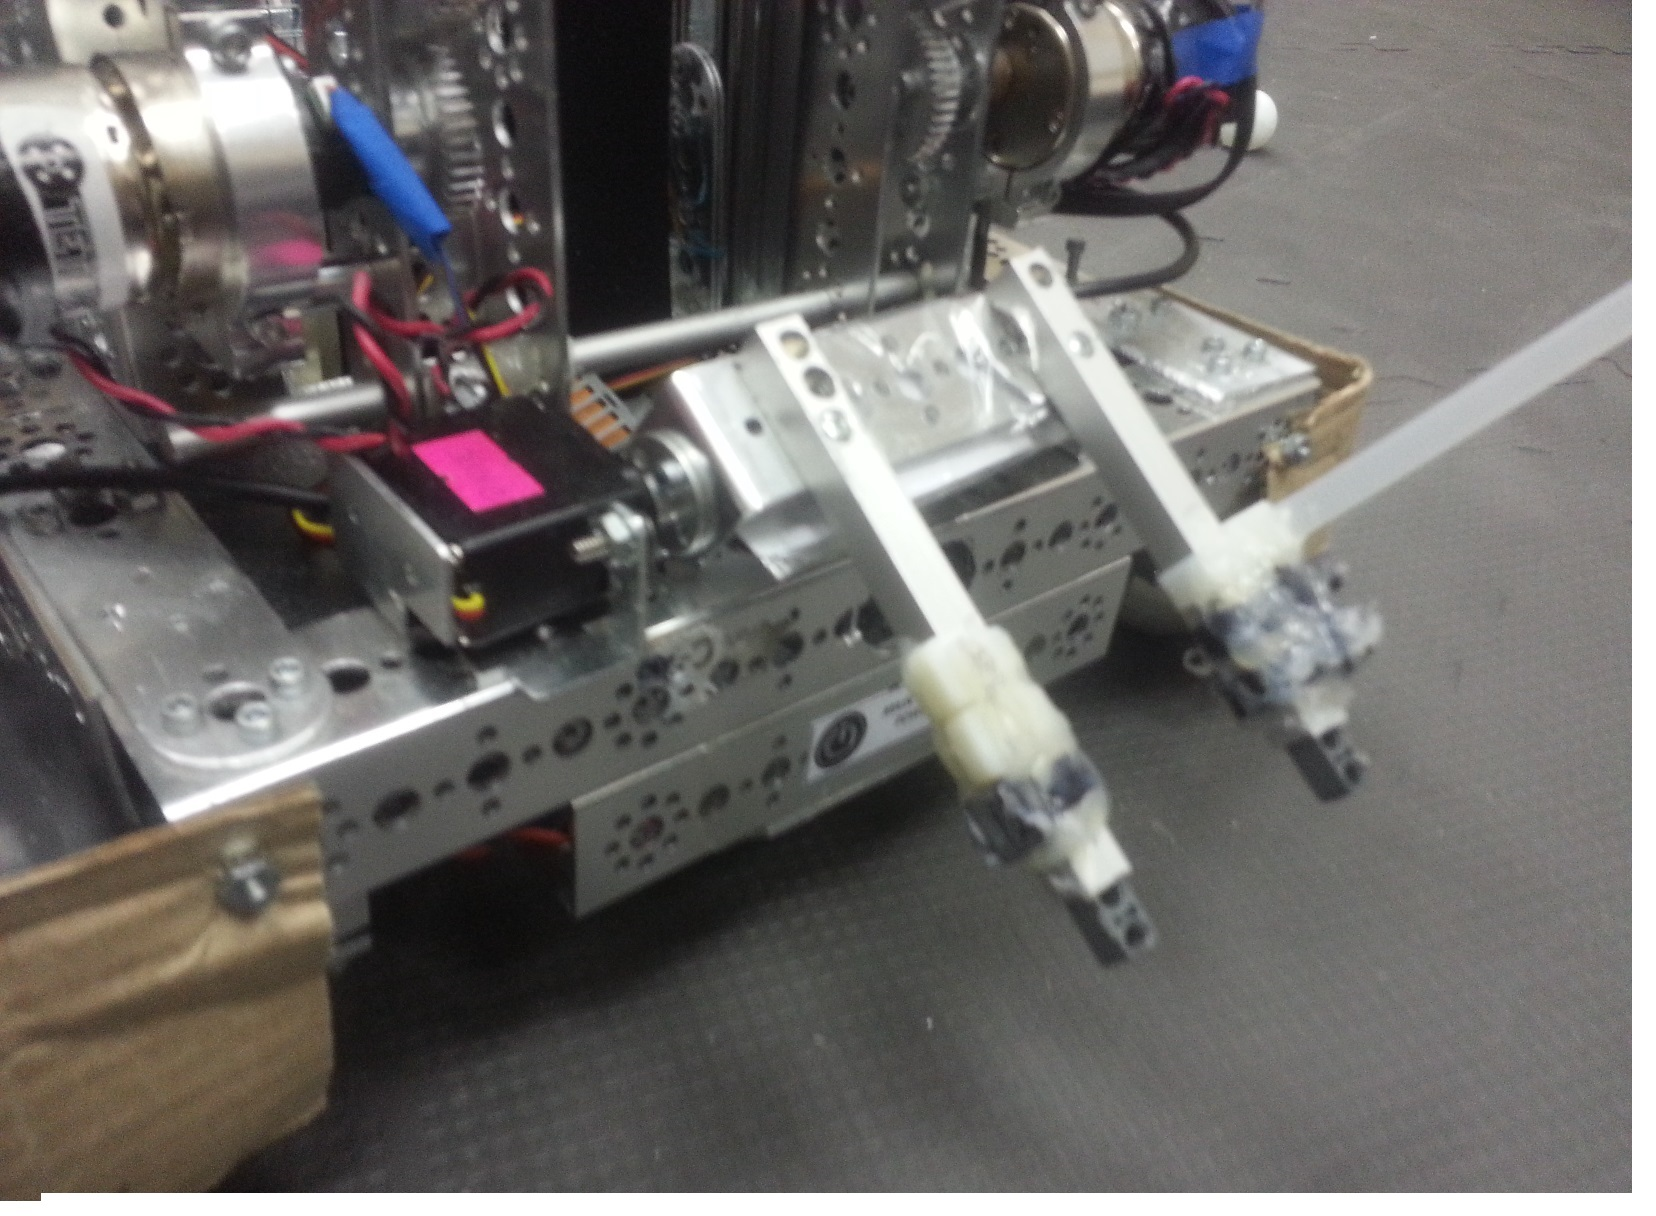
\includegraphics[scale=0.3]{days/22.11.14/images/01}}
%			\caption{Укрепление перекладины}
%		\end{minipage}
%	\end{figure}
	
	\item На механизм захвата корзин были установлены откосы из стяжек для центровки захватываемой нами корзины. В дальнейшем планируется заменить стяжки  пластиковыми полосами, т.к. они часто ломаются.
	
	\begin{figure}[H]
		\begin{minipage}[h]{0.2\linewidth}
			\center  
		\end{minipage}
		\begin{minipage}[h]{0.6\linewidth}
			\center{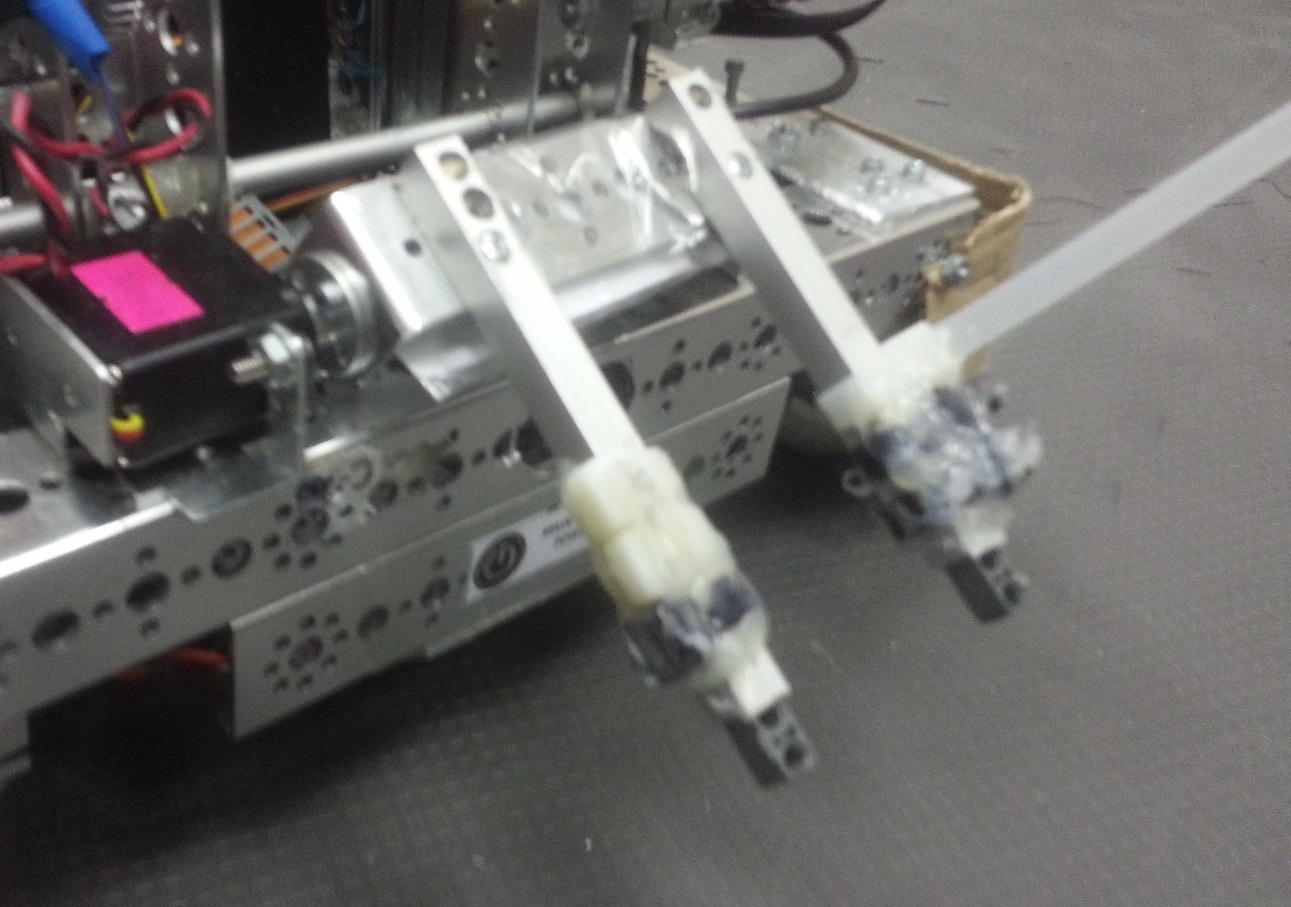
\includegraphics[scale=0.15]{days/22.11.14/images/02}}
			\caption{Откосы для центровки корзины (на фотографии 6 из 5 стяжек сломаны).}
		\end{minipage}
	\end{figure}
	
	\item Защита от попадания мячей под колеса была улучшена. На данный момент защита картонная, но после возвращения с соревнований мы сделаем ее металлической.
	
	\begin{figure}[H]
		\begin{minipage}[h]{0.2\linewidth}
			\center  
		\end{minipage}
		\begin{minipage}[h]{0.6\linewidth}
			\center{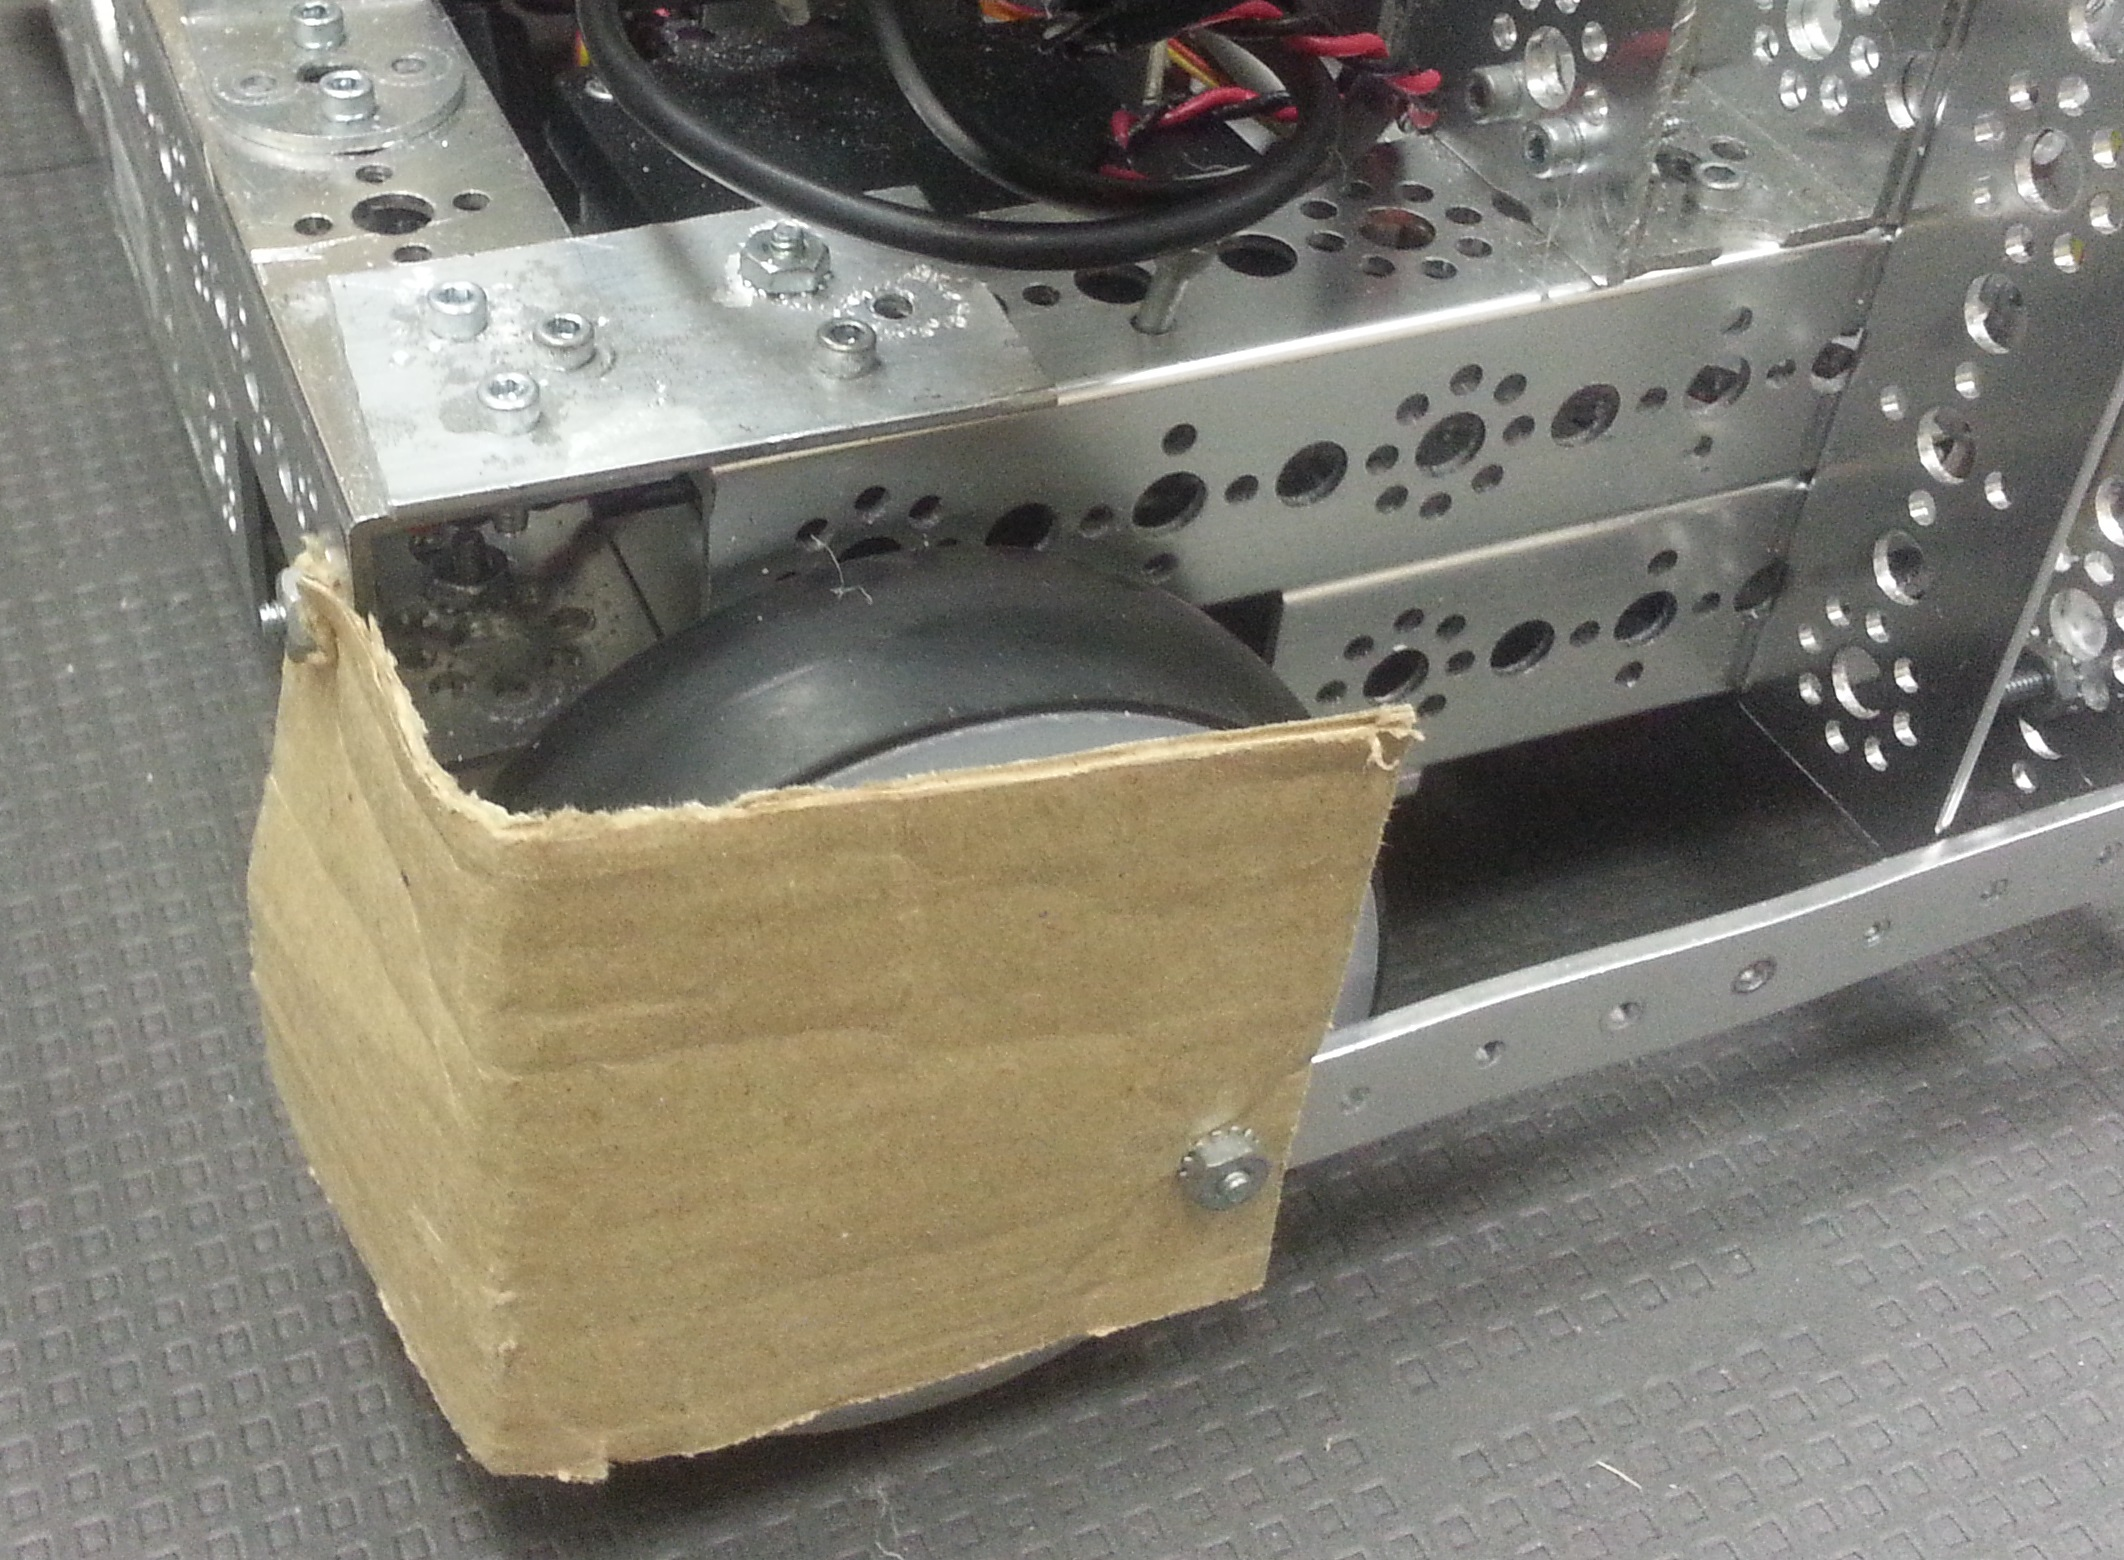
\includegraphics[scale=0.1]{days/22.11.14/images/03}}
			\caption{Защита задних колес}
		\end{minipage}
	\end{figure}
	
	\item В связи с тем, что NXT-блок во время одного из заездов отвалился от робота, мы закрепили его как можно надежнее.
	
	\begin{figure}[H]
		\begin{minipage}[h]{0.2\linewidth}
			\center  
		\end{minipage}
		\begin{minipage}[h]{0.6\linewidth}
			\center{
\includegraphics[scale=0.2]{days/22.11.14/images/04}}
			\caption{Улучшенная фиксация NXT-блока}
		\end{minipage}
	\end{figure}
	
	\item Было замечено, что во время раздвигания подъемника верхняя пара мебельных реек раздвигалась в последнюю очередь, что не давало возможности опрокидывать ковш до тех пор, пока подъемник не будет полностью раздвинут. Эта проблема отнимала много времени на совершение лишних дыижений, поэтому было решено по возвращении с соревнований каким-то образом устранить эту проблему.
	
\end{enumerate}
\fillpage